\section{Data}
\label{sec:data}
\label{app:ext_data}
\emph{In short: the record, the common preselection and the fit window; the spectrum peaks at $5284\,\MeV$ for both charges and both polarities, and the counting asymmetry is $-0.043\pm0.007$.}
\subsection{Dataset, Preselection and Mass}
\label{sec:data_presel}
\emph{In short: $8{,}556{,}118$ candidates are reduced to $23{,}895$ by a kaon-identification and muon-veto requirement common to the analyses; the fit window $[5100,5600]\,\MeV$ contains $19{,}731$ candidates ($10{,}292$ $B^+$, $9439$ $B^-$).}
The dataset is the CERN Open Data record 4900~\cite{opendata_record}: $B^{\pm}\to h^{\pm}h^{+}h^{-}$ candidates collected by LHCb in 2011 at $\sqrt{s}=7$\,TeV, already through trigger and offline selection, distributed as ROOT \texttt{TTree}s with the most relevant branches and split by magnet polarity, for $8{,}556{,}118$ candidates. The record also contains a phase-space simulation of $B^{\pm}\to K^{\pm}K^{+}K^{-}$ ($50{,}000$ decays, no asymmetry), used only to test the local-asymmetry procedure (Sec.~\ref{sec:dalitz}).
For each of the three final-state tracks ($H1$, $H2$, $H3$) the analysis reads the momentum components, the particle-identification (PID) likelihoods (\texttt{ProbK}, \texttt{ProbPi}), a muon flag and the charge. The same preselection is used in all analyses,
\[
\texttt{H*\_ProbPi} < 0.5 \ \wedge\ \texttt{H*\_ProbK} > 0.5 \ \wedge\ \lnot\texttt{H*\_isMuon},
\]
and retains $23{,}895$ of the $8{,}556{,}118$ candidates ($0.28\%$), the PID requirement being the dominant reduction (Table~\ref{tab:cutflow}).

\begin{table}[h]
\centering
\resizebox{\ifdim\width>\linewidth\linewidth\else\width\fi}{!}{\begin{tabular}{lrrrr}
\toprule
Requirement & alone & cumulative & down & up \\
\midrule
All candidates & -- & $8{,}556{,}118$ & $5{,}135{,}823$ & $3{,}420{,}295$ \\
$\lnot\texttt{isMuon}$, three tracks & $6{,}311{,}517$ & $6{,}311{,}517$ & $3{,}806{,}297$ & $2{,}505{,}220$ \\
$\texttt{ProbPi}<0.5$, three tracks & $975{,}724$ & $481{,}101$ & $288{,}908$ & $192{,}193$ \\
$\texttt{ProbK}>0.5$, three tracks & $28{,}812$ & $23{,}895$ & $14{,}178$ & $9717$ \\
Mass window $[5100,5600]\,\MeV$ & -- & $19{,}731$ & $11{,}636$ & $8095$ \\
\bottomrule
\end{tabular}}
\caption{Number of candidates passing each requirement alone and after the cumulative selection, in the order of the table, and by magnet polarity. The kaon-identification requirement on the three tracks is by far the most selective.}
\label{tab:cutflow}
\end{table}

$H1$ is always the kaon of charge opposite to the $B$, so the Dalitz variables are $m^2(H1,H2)$ and $m^2(H1,H3)$.
\label{sec:data_mass}
The three final-state tracks are assigned the charged-kaon mass hypothesis ($M_K=493.677\,\MeV$) regardless of their PID likelihoods, and their four-momenta are summed to reconstruct the $B$ candidate, $m(KKK)=\sqrt{(\sum_i E_i)^2-|\sum_i \vec{p}_i|^2}$. The nominal fit window, common to the Frequentist and Bayesian analyses, is $[5100,5600]\,\MeV$ and contains $19{,}731$ candidates ($10{,}292$ $B^+$, $9439$ $B^-$; $11{,}636$ magnet down, $8095$ magnet up). Below $\sim$5150\,\MeV\ the background rises, consistent with a partially reconstructed contribution that a single exponential cannot describe; the window includes the start of this rise, which is described by a second exponential in the background model (Secs.~\ref{sec:frequentist}--\ref{sec:bayesian}). The machine-learning selection (Sec.~\ref{sec:ml}) uses the same window.
\subsection{Data Exploration}
\label{sec:data_exploration}
\emph{In short: the spectrum peaks at $5284\,\MeV$ with a similar shape for the two charges and the two magnet polarities, and the counting asymmetry of all candidates is $-0.043\pm0.007$.}

Figure~\ref{fig:mass_spectrum} shows the spectrum in the fit window, split by $B$ charge (a) and by magnet polarity (b). The peak at $m\approx5284\,\MeV$ over a falling combinatorial background has the same shape for the two charges and for the two polarities, which is what allows a mass and a resolution common to $B^+$ and $B^-$ in the model (Sec.~\ref{sec:model}). The asymmetry itself is not visible by eye: the counting asymmetry of all candidates, signal and background together, is $A_{\mathrm{count}}=(N^--N^+)/(N^-+N^+)=-0.043\pm0.007$ (binomial uncertainty), and the fits of Secs.~\ref{sec:frequentist} and \ref{sec:bayesian} refine it by separating signal and background.

\begin{figure}[t]
\centering
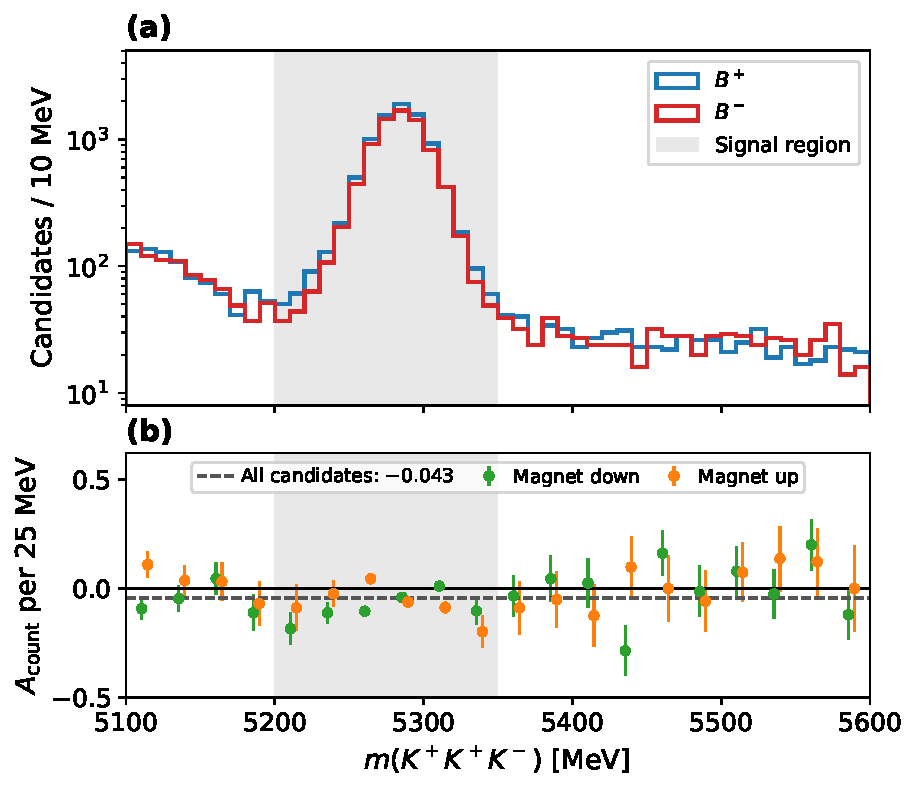
\includegraphics[width=\columnwidth]{figures/mass_spectrum_col.pdf}
\caption{(a) Reconstructed $B\to KKK$ invariant mass in the nominal fit window $[5100,5600]\,\MeV$ for $B^+$ and $B^-$, logarithmic scale; the signal region $[5200,5350]\,\MeV$ is shaded. (b) Counting asymmetry in $25\,\MeV$ bins of the mass for the two magnet polarities, and for all candidates (dashed); the two polarities agree within their uncertainties and the asymmetry is similar in the peak and in the sidebands.}
\label{fig:mass_spectrum}
\end{figure}

\subsection{Cut Flow of the Preselection}
\label{app:cutflow}
\emph{In short: the kaon-identification requirement on the three tracks is by far the most selective.}

\subsection{Candidates Sharing a Track}
\emph{In short: only $42$ candidates of the fit window ($0.2\%$) share a track with another candidate, a negligible effect, and all are kept.}
The files have no event identifier; only $42$ candidates of the fit window ($0.2\%$) share a track with another candidate, a negligible effect, and all are kept.
\subsection{Charge Combinations}
\emph{In short: $H1$ is always the kaon of charge opposite to the $B$ and $H2$, $H3$ the same-sign pair, so the Dalitz variables are the two opposite-sign invariant masses.}
In this dataset only the charge combinations $(+1,-1,-1)$ and $(-1,+1,+1)$ occur for $(H1,H2,H3)$: $H1$ is always the kaon of charge opposite to the $B$, and $H2$, $H3$ are the interchangeable same-sign pair. The Dalitz-plot variables are therefore the invariant masses of the two opposite-sign pairs, $m^2(H1,H2)$ and $m^2(H1,H3)$.
